\chapter{Measurement of Angles}
The word trigonometry comes from means measurement of triangles. The word originally comes from Greek language.
measurement. The objective of studying plane trigonometry is to develop a method of solving plane triangles. However, as time
changes everything it has changed the scope of trigonometry to include polygons and circles as well. A lot of concepts in this book
will come from your geometry classes in lower classes. It is a good idea to review the concepts which you have studied till now
without which you are going to struggle while studying trigonometry in this book.

\section{Angles in Geometry}
If we consider a line extending to infinity in both directions, and a point $OO$ which divides this line in two parts one on each
side of the point then each part is called a ray or half-line. Thus $O$ divides the line into two rays $OA$ and $OA'$.

\begin{center}
  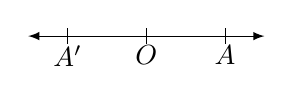
\begin{tikzpicture}
    \draw[>=latex,<->] (0, 0) -- (3, 0);
    \draw (.5, -.1) -- (.5, .1);
    \draw (.5,0) node[anchor=north] {$A'$};
    \draw (2.5, -.1) -- (2.5, .1);
    \draw (2.5,0) node[anchor=north] {$A$};
    \draw (1.5, -.1) -- (1.5, .1);
    \draw (1.5,0) node[anchor=north] {$O$};
  \end{tikzpicture}
\end{center}

The point $O$ is called vertex or origin for these days. An angle is a figure formed by two rays or half lies meeting at a common
vertex. These half lines are called {\it sides of the angle}.

An angle is denoted by the symbol $\angle$ followed by three capital letters of which the middle one represents the vertex and
remaining two points point to two sides. Otherwise the angle is simply written as one letter representing the vertex of the
angle.

\begin{center}
  \begin{tikzpicture}
    \draw[->, >=stealth] (0,0) -- (2,0);
    \draw[->, >=stealth] (0,0) -- (1, 1.732);
    \draw (0.3, 0) arc [start angle=0, end angle=60, radius=0.3];
    \draw (2, 0) node[anchor=north] {$A$};
    \draw (1, 1.732) node[anchor=north west] {$B$};
    \draw (0, 0) node[anchor=north] {$O$};
  \end{tikzpicture}
\end{center}


The angle in above image is written as $\angle AOB$ or $\angle BOA$ or $\angle O$.

Each angle can be measured and there are different units for the measurement. In Geometry, an angle always lie between $0^\circ$
and $360^\circ$ and negative angles are meaningless. Measure of an angle is the smallest amount of rotation from the direction of
one ray of the angle to the direction of the other.

\section{Angles in Trigonometry}
Angles are more generalized in Trigonometry. They can have positive or negative values. As was the case in gerometry, similarly
angles are measured in Trigonometry. The starting and ending positions of revolving rays are called initial side and terminal side
respectively. The revolving half line is called the generating line or the radius vector. For example, if $OA$ and $OB$ are the
initial and final position of the radius vector then angle formed will be $\angle AOB$.

\section{Angles Exceeding $360^\circ$}
\begin{center}
  \begin{tikzpicture}
	  \draw [->]( 0,0) -- (4,0);
	  \draw [->]( 0,0) -- (0,4);
	  \draw [->,red]( 0,0) -- (400:4);
    \draw[->,domain=0:400,variable=\t,samples=200,>=latex]
    plot ({(\t+400)*cos(\t)/(400)},
    {(\t+400)*sin(\t)/(400)}) node[right=.5cm] {$400^\circ$};
  \end{tikzpicture}
\end{center}

In Geometry, angles are limited to $0^\circ$ to $360^\circ$. However, when multiple revolutions are involved angles are more than
$360^\circ$. For example, the revolving line starts from the initial position and makes $n$ complete revolutions in anticlockwise
direction and also further angle $\alpha$ in the same direction. We then have a certain angle $\beta_n$ given by $\beta_n =
x\times360^\circ + \alpha$, where $0^\circ< \alpha < 360^\circ$ and $n$ is zero or positive integer. Thus, there are infinite
possible angles.

Angles formed by anticlockwise rotation of the radius vector are taken as positive and angles formed by clockwise rotation of the
radius vector are taken as negative.

\section{Quadrants}
\begin{center}
  \begin{tikzpicture}
    \draw[>=latex,<->] (0, 0) -- (3, 0);
    \draw (0,0) node[anchor=north] {$X'$};
    \draw (3,0) node[anchor=north] {$X$};
    \draw (1.5,0) node[anchor=north east] {$O$};
    \draw[>=latex,<->] (1.5, -1.5) -- (1.5, 1.5);
    \draw (1.5, -1.5) node[anchor=west] {$Y'$};
    \draw (1.5, 1.5) node[anchor=west] {$Y$};
  \end{tikzpicture}
\end{center}

Let $XOX'$ and $YOY'$ be two mutually perpendicular lines in a plane and $OX$ be the initial half line. The lines divide the whole
reason in quadrants. $XOY, YOX', X′OY$' and $Y′OX$ are respectively called $1$st, $2$nd, $3$rd and $4$th quadrants. According to
terminal side lying in $1$st, $2$nd, $3$rd and $4$th quadrants the angles are said to be in $1$st, $2$nd, $3$rd and $4$th quadrants
respectively. A {\it quandrant angle} is an angle formed if terminal side coincides with one of the axes.

For any angle $\angle$ which is not a quadrant angle and when number of revolutions is zero and radius vector rotates in
anticlockwise directions:

\begin{enumerate}
\item $0^\circ< \alpha < 90^\circ$ if $\alpha$ lies in first quadrant
\item $90^\circ< \alpha < 180^\circ$ if $\alpha$ lies in second quadrant
\item $180^\circ< \alpha < 270^\circ$ if $\alpha$ lies in third quadrant
\item $270^\circ< \alpha < 360^\circ$ if $\alpha$ lies in fourth quadrant
\item when terminal side lies on $OY$, angle formed $=90^\circ$
\item when terminal side lies on $OX'$, angle formed $=180^\circ$
\item when terminal side lies on $OY'$, angle formed $=270^\circ$
\item when terminal side lies on $OX$, angle formed $=360^\circ$
\end{enumerate}

\section{Units of Measurement}
In Geometry, angles are usually measured in terms of right angles, however, that is an inconvenient system for smaller angles. So
we introduce different systems of measurements. There are three system of units for this:

\begin{enumerate}
\item Sexagecimal or British system: In British system, a right angle is divided into $90$ equal parts called degrees. Each degree
is then divided into $60$ equal parts called minutes and each minute is further is divided into $60$ parts called seconds.

A degree, a minute and a second are denoted by $1^\circ, 1"$, and $1$ respectively.
\item Centesimal or French System: In French system, a right angle is divided into $100$ equal parts called grades. Each grade is
then divided into $100$ equal parts called minutes and each minute is further is divided into $100$ parts called seconds.

A degree, a grade and a second are denoted by $1^g, 1"$, and $1$ respectively.
\item Radian or Circular Measure: An arc equal to radius of a circle when subtends an anngle on the center then that angle is $1$
radian and is denoted by $1^c$. The angle made by half of perimeter is $\pi$ radians. Also, from Geometry we know that angle subtended
is the ratio between length of cord and radius. This ratio is in radians. Since both length or chord and radius have same unit
radian is a constant.
\end{enumerate}

\subsection{Relationship between Systems of Measurements}
If measure of an angle if $D$ degrees, $G$ grades and $C$ radians then upon elementary manipulation we find that $\frac{D}{180}=
\frac{G}{200} = \frac{C}{\pi}$.

\subsection{Meaning of $\pi$}
The ratio of circumference and diameter of a circle is always constant and this constant is denoted by gree letter $\pi$.

$\pi$ is an irrational number. In general, we use the value of $\frac{22}{7}$ but $\frac{355}{113}$ is more accurate though not
exact. If $r$ be the radius of a circle and $c$ be the circumference then $\frac{c}{2r} =\pi$ leading circumference to be $c = 2\pi
r$.

\section{Problems}
\begin{enumerate}
\item Reduce $63^{\circ}14'51''$ to centisimal measure.
\item  Reduce $`45^{\circ}20'10''$ to centisimal and radian measure.
\item Reduce $94^g23'27''$ to Sexagecimal measure.
\item Reduce $1.2$ radians in Sexageciaml measure.
\end{enumerate}

Express in terms of right angle; the angles

\begin{enumerate}[resume]
\item $60^{\circ}$
\item $75^{\circ}15'$
\item $63^{\circ}17'25''$
\item $130^{\circ}30'$
\item $210^{\circ}30'30''$
\item $370^{\circ}20'48''$
\end{enumerate}

Express in grades, minutes and degrees

\begin{enumerate}[resume]
\item $30^{\circ}$
\item $81^{\circ}$
\item $138^{\circ}30'$
\item $35^{\circ}47'15''$
\item $235^{\circ}12'36''s$
\item $475^{\circ}13'48''$
\end{enumerate}

Express in terms of right angles and also in degrees, minutes and seconds; the angles

\begin{enumerate}[resume]
\item $120^g$
\item $45^g35'24''$
\item $39^g45'36''$
\item $255^g8'9''$
\item $759^g0'5''$
\item Reduce $55^{\circ}12'36''$ to centisimal measure.
\item Reduce $18^{\circ}33'45''$ to circular measure.
\item Reduce $196^g35'24''$ to sexagecimal measure.
\item How many degrees, minutes and seconds are respectively passed over in $11\frac{1}{9}$ minutes by the hour and minute hand
    of a watch.
\item The number of degrees in one acute angle of a right-angled triangle is equal to the number of grades in the other; express both
    angles in degrees.
\item Prove that the number of Sexagecimal minutes in any angle is to the number of Centisimal minutes in the same angle as
    $27:50.$
\item Divide $44^{\circ}8'$ into two parts such that the number of Sexagecimal seconds in one part may be equal to number of
    Centisimal seconds in the other part.
\item The angles of a triangle are in the ratio of $3:4:5$, find the smallest angle in degrees and greatest angle in radians.
\item Find the angle between the hour hand and the minute hand in circular measure at half past four.
\item If $p, q$ and $r$ denote the grade measure, degree measure and the radian measure of the same angle, prove that
  \begin{enumerate}
    \item $\frac{p}{10} = \frac{q}{9} = \frac{20r}{\pi}$
    \item $p - q = \frac{20r}{\pi}$
  \end{enumerate}
\item Two angles of a triangle are $72^{\circ}53'51''$ and $41^{\circ}22'50''$ respectively. Find the third angle in
    radians.
\item The angles of triangle are in A.P. and the number of radians in the greatest angle is to the number of degrees in the least one
    as $\pi:60$; find the angles in degrees.
\item The angles of a triangle are in A.P. and the number of grades in the least is to the number of radians in the greatest is
$40:\pi$; find the angles in degrees.
\item Three angles are in G.P. The number of grades in the greatest angle is to the number of circular units in the least is
    $800:\pi$; and the sum of angles is $126^\circ$. Find the angles in grades.
\item Find the angle between the hour-hand and minute-hand in circular measure at $4$ o'clock.
\item Express in sexagecimal system the angle between the minute-hand and hour-hand of a clock at quarter to twelve.
\item The diamter of a wheel is $28$ cm; through what distance does its center move during one rotation of wheel along the
    ground?
\item What must be the radius of a circular running path, round which an athlete must run $5$ time in order to describe
    $1760$ meters?
\item The wheel of a railway carriage is $90$ cm in diameter and it makes $3$ revolutions per second; how fast is the
    train going?
\item A mill sail whose length is $540$ cm makes $10$ revolutions per minute. What distance does its end travel in one
    hour?
\item Assuming that the earth describes in one year a circle, or $149,700,000$ km. radius, whose center is the sun, how many
    miles does earth travel in a year?
\item The radius of a carriage wheel is $50$ cm, and in $\frac{1}{9}$ th of a second it turns through $80^\circ$
    about its center, which is fixed; how many km. does a point on the rim of the wheel travel in one hour?
\item Express in terms of three systems of angular measurements the magnitude of an angle of a regular decagon.
\item One angle of a triangle is $\frac{2}{3}x$ grades and another is $\frac{3}{2}x$ degrees, while the third is
    $\frac{\pi x}{75}$ radians; express them all in degrees.
\item The circular measure of two angles of a triangle are $\frac{1}{2}$ and $\frac{1}{3}$. What is the number of degrees
    of the third angle?
\item The angles of a triangle are in A.P. The number of radians in the least angle is to the number of degree in the mean angle is
    $1:120$. Find the angles in radians.
\item Find the magnitude, in radians and degrees, of the interior angle of 1. a regular pentagon 2. a regular heptagon 3. a regualr
    octagon 4. a regular duodecagon 5. a polygon with $17$ sides
\item The angle in one regular polygon is to that in another is $3:2$, also the number of sides in the first is twice that in
    the second. How many sides are there in the polygons?
\item The number of sides in two regular polygons are as $5:4$, and the difference between their angles is $9^\circ$;
    find the number of sides in the polygons.
\item Find two regular polygons such that the number of their sides may be $3$ to $4$ and the number of degrees of an
    angle of the first to the number of grades of the second as $4$ to $5.$
\item The angles of a qadrilateral are in A.P. and the greatest is double the least; express the least angle in radians.
\item Find in radians, degrees, and grades the angle between hour-hand and minute-hand of a clock at 1. half-past three 2. twenty
    minutes to six 3. a quarter past eleven.
\item Find the times 1. between fours and five o'clock when the angle between the minute hand and the hour-hand is
    $78^\circ,$ 2. between seven and eight o'clock when the angle is $54^\circ$
\item The interior angles of a polygon are in A.P. The smallest angle is $120^\circ$ and the common difference is
    $5^\circ$. Find the number of sides of the polygon.
\item The angles of quadrilateral are in A.P. and the number of grades in the least angle is to the number of radians in the greatest is
    $100:\pi$. Find the angles in degrees.
\item The anlges of a polygons are in A.P. The least angle is $\frac{5\pi}{12}$ common difference is $10^\circ$, find the
    number of sides in the polygon.
\item Find the angle subtended at the center of a circle of radius $3$ cm. by an arc of length $1$ cm.
\item In a circle of radius $5$ cm., what is the length of the arc which subtends an angle of $33^\circ15'$ at the center.
\item Assuming the average distance of sun from the earth to be $149,700,000$ km., and the angle subtended by the sun at the
    eye of a person on the earth is $32'$, find the sun's diameter.
\item Assuming that a person of normal sight can read print at such a distance that the letter subtends and angle of $5'$ at
    his eye, find what is the height of the letters he can read at a distance of 1. $12$ meters 2. $1320$ meters.
\item Find the number of degrees subtended at the center of a circle by an arc whose length is $0.357$ times the radius.
\item Express in radians and degrees the angle subtended at the center of a circle by an arc whose length is $15$ cm., the
    radius of the circle being $25$ cm.
\item The value of the divisions on the outer rim of a graduated cicle is $5'$ and the distance between successive graduations
    is $.1$ cm. Find the radius of the circle.
\item The diamter of a graduated circle is $72$ cm., and the gradiuations on the rim are $5'$ apart; find the distance of
    one graduation to to another.
\item Find the radius of a globe which is such that the distance between two places on the same meridian whose latitude differs by
    $1^\circ10'$ may be $0.5$ cm.
\item Taking the radius of earth to as $6400$ km., find the difference in latitude of two places, one of which is $100$
    km. north of another.
\item Assuming the earth to be a sphere and the difference between two parallels of latitude, which subtends an angle of
    $1^\circ$ at the eath's center, to be $69\frac{1}{2}$ km., find the radius of the earth.
\item What is the ratio of radii of the circles at the center of which two arcs of same length subtend angles of $60^\circ$ and
    $75^\circ$?
\item If an arc, of length $10$ cm., on a circle of $8$ cm. diameter subtend at the center of circle an angle of
    $143^\circ14'22''$, find the value of $\pi$ to $4$ places of decimals.
\item If the circumference of a circle be divided into five parts which are in A.P., and if the greatest part be six times the least
    find in radians the the magnitude of the angles the parts subtend at the center of the circle.
\item The perimeter of a certain sector of a circle is equal to the length of the arc of a semicircle having the same radius; express
    the angle of the sector in degrees.
\item At what distance a man, whose height is $2$ m., subtend an angle of $10'$.
\item Find the length which at a distance of $5280$ m., will subtend an angle of $1'$ at the eye.
\item Assuming the distance of the earth from the moon to be $38400$ km., and the angle subtended by the moon at the eye of a
    person on earth to be $31'$, find the diameter of the moon.
\item The wheel of a railway carriage is $4$ ft. in diameter and makes $6$ revolutions in a second; how fast is the train
    going?
\item Assuming that moon subtends an angle of $30'$ at the eye of an observer, find how far from the eye a coin of one inch
    diameter must be held so as just to hide the moon.
\item A wheel make $30$ revolutions per minute. Find the circular measure of the angle described by spoke in half a second.
\item A man running along a circular track at the rate of $10$ miles per hour, traverses in $36$ seconds, an arc which
    subtends an angle of $56^\circ$ at the center. Find the diamter of the circle.
\end{enumerate}
